% =====================================================================
% RASCUNHO de revisão — comentários do Cleber (21/out), 2ª versão.
% Arquivo novo timestamped; NÃO sobrescreve main.tex.
% Status: números da Fase B/C já computados (n=3, exploratório).
% TODO(verificar): referências de related work (SunGen) e curadoria humana.
% =====================================================================
\documentclass[conference]{IEEEtran}
\usepackage[utf8]{inputenc}
\usepackage[T1]{fontenc}
\usepackage{cite}
\usepackage{amsmath,amssymb,amsfonts}
\usepackage{graphicx}
\usepackage{textcomp}
\usepackage{xcolor}
\usepackage{booktabs}
\usepackage[hidelinks]{hyperref}
\usepackage{url}
\usepackage{balance}
\usepackage{enumitem}
\graphicspath{{./images/}{../figures/revision/}{./}}
\setlist{nosep,leftmargin=*}
\setlength{\textfloatsep}{6pt plus 1pt minus 1pt}
\setlength{\intextsep}{5pt plus 1pt minus 1pt}
\setlength{\floatsep}{5pt plus 1pt minus 1pt}
\widowpenalty=10000
\clubpenalty=10000

\begin{document}

\title{Geração Sintética Guiada por Herança Ativa para Detecção de Desinformação}

\author{
\IEEEauthorblockN{Eduardo Alexandre de Amorim\textsuperscript{1}, Cleber Zanchettin\textsuperscript{1}}
\IEEEauthorblockA{\textsuperscript{1}Centro de Informática, Universidade Federal de Pernambuco, Recife, PE, Brasil\\
\{eaa5, cz\}@cin.ufpe.br}
}

\maketitle

\begin{abstract}
A escassez de exemplos rotulados limita classificadores de desinformação, e a geração sintética indiscriminada pode introduzir redundância, artefatos e ruído. Este trabalho revisa o \emph{ActiveInheritance} como um estudo controlado de curadoria: dados os mesmos candidatos gerados por um modelo de linguagem, o que vale a pena herdar para treinar o classificador downstream? Comparamos quatro regras sobre os mesmos lotes em português---herdar tudo (\emph{All}), uma amostra aleatória (\emph{Random-}k), o score de erro/incerteza/diversidade (\emph{Score-}k) e o gate invertido (\emph{Easy-}k)---em três cenários temporais do FakeWhatsApp.Br. Também reavaliamos os pools antigos com ponderação de classes e limiar ajustado na validação, além de PR-AUC/ROC-AUC. Resultados (três seeds, exploratório) mostram que o score não domina a seleção aleatória: \emph{Random-}k empata no cenário completo e lidera sob escassez (10\% e 5\%). A ponderação de classes e o limiar recuperam o recall que antes colapsava (Real 5\%: F1 de $0{,}000$ para $0{,}642$). Concluímos que o benefício observado é curadoria de volume e calibração de treino, não o score em si.
\end{abstract}

\begin{IEEEkeywords}
data-centric AI, synthetic data, misinformation detection, active learning, controlled study, large language models, Portuguese NLP
\end{IEEEkeywords}

\section{Introdução}

A detecção automática de desinformação em português é limitada por escassez de exemplos positivos, mudança de domínio e custo de anotação. Modelos de linguagem permitem gerar dados sintéticos, mas volume não garante utilidade: gerações repetem templates, afastam-se da distribuição real ou recebem rótulos presumidos incorretos~\cite{shumailov2024}.

A versão anterior deste trabalho propôs o \emph{ActiveInheritance}: herdar ciclicamente os candidatos com maior erro, incerteza e diversidade. Os resultados, porém, misturavam três efeitos---o score, o volume gerado e a sequência de retreinos---e usavam limiar fixo de $0{,}5$ sem ponderação de classes, o que confundia qualidade sintética com política de treino. Esta revisão isola esses fatores. As perguntas de pesquisa são:

\begin{enumerate}
\item[\textbf{RQ1}] (qualidade) Dados os mesmos candidatos, selecionar por erro/incerteza/diversidade produz dados mais úteis que uma seleção aleatória?
\item[\textbf{RQ2}] (eficiência) Herdar um subconjunto curado é melhor que usar toda a geração, em função do número de sintéticos e de tokens?
\item[\textbf{RQ3}] (robustez) Quanto do colapso de recall sob escassez é efeito do limiar fixo e do desbalanceamento, e não do gate?
\end{enumerate}

A contribuição é um \textbf{estudo controlado de curadoria} em português e split temporal: quatro braços sobre os \emph{mesmos} candidatos zero-shot, com ponderação de classes, limiar ajustado na validação, PR-AUC/ROC-AUC e treino final do zero.

\textbf{Trabalhos relacionados.} O trabalho se insere em \emph{data-centric AI} e em \emph{active learning}~\cite{settles2012}. A literatura de geração sintética zero-shot (e.g., ZeroGen e ProGen) gera exemplos para treinar modelos; a \emph{Dataset Cartography}~\cite{swayamdipta2020} diagnostica a dificuldade de exemplos pela dinâmica de treino. Nosso estudo não propõe novo gerador nem novo score: mede, de forma controlada, \emph{quando} uma regra de seleção ajuda---em português e com split temporal. % TODO(verificar): citar ZeroGen/ProGen/SunGen com autores e veículo confirmados antes de submeter.

\section{Método}

\subsection{Loop e score}

Dado um treino real $D_0$, um learner $f$ e um pool herdado $H$, um gerador produz um lote $S_t$ por ciclo. Para cada texto $x$, o avaliador calcula

\begin{equation}
 s(x)=w_e\,e(x)+w_u\,u(x)+w_d\,d(x),
 \label{eq:score}
\end{equation}

onde $e$ é o log-loss presumindo rótulo \texttt{fake}, $u$ é a entropia binária normalizada e $d$ é a diversidade (um menos a maior similaridade de cosseno contra $H$, com MiniLM multilíngue). Configuração: $(w_e,w_u,w_d)=(0{,}4,0{,}4,0{,}2)$, $T=5$, batch $64$, top-$k=16$.

\subsection{Quatro braços sobre os mesmos candidatos}

\begin{itemize}
\item \textbf{All}: herda todos os candidatos de cada lote.
\item \textbf{Random-}k: herda $k$ candidatos sorteados (controle para o efeito do score).
\item \textbf{Score-}k: herda o top-$k$ pela Eq.~\eqref{eq:score}.
\item \textbf{Easy-}k: herda o \emph{bottom}-$k$ pela Eq.~\eqref{eq:score} (inversão estilo Profile2Gen~\cite{souza2025}, que remove hard samples).
\end{itemize}

\subsection{Protocolo corrigido}

(i) geração \textbf{zero-shot} (sem exemplos herdados) para que os quatro braços compartilhem os mesmos lotes; (ii) \textbf{ponderação de classes} em todos os braços, incluindo o treino real; (iii) \textbf{limiar ajustado na validação} (não fixo em $0{,}5$) e reporte de PR-AUC/ROC-AUC; (iv) treino final de um BERT \textbf{novo} em $D_0\cup H$; (v) registro de tokens de entrada/saída e custo. O pool antigo guardava apenas herdados; por isso os braços Random/Easy/Score/All desta revisão usam geração nova com candidatos completos salvos.

\section{Configuração Experimental}

Usamos o FakeWhatsApp.Br~\cite{cabral2021} (6.926 mensagens únicas, rótulo manual), texto raw e split temporal: julho--agosto (treino), setembro (validação) e outubro (teste). Cenários: \emph{full} (474 fake/683 true), \emph{10\%} (47/683) e \emph{5\%} (23/683). Learner BERTimbau~\cite{souza2020}, três épocas por fit, batch 16, comprimento 256; gerador \texttt{deepseek-chat}, prompt v4 (anti-template), teto de 100 mil tokens por geração. Seeds 42--44. Com três seeds, o Wilcoxon bilateral não atinge $p<0{,}05$; os resultados são exploratórios.

A Fase B re-treina BERTimbau do zero nos pools sintéticos \emph{já salvos} (zero API) com ponderação e limiar, comparando ao protocolo antigo (limiar $0{,}5$, sem pesos).

\textbf{Seeds.} Para o WhatsApp, treino/validação/teste são fixos; a seed muda a inicialização do BERT e a ordem de treino, além da estocasticidade da geração LLM (que não é determinística no servidor). No Fake.br antigo, a seed também dividia treino/validação; na revisão, criamos uma validação fixa (80/20 estratificado, seed 42) para não escolher método olhando o teste.

\textbf{Custo.} A geração é zero-shot e compartilhada pelos quatro braços: 9 gerações completas somaram $895.512$ tokens ($321.435$ de entrada e $574.077$ de saída), custo estimado de US\$0{,}72 pelos preços do código (aproximados; conferir fatura do provedor). O protocolo antigo do AI consumia $\approx$2 mil tokens por candidato porque o prompt carregava exemplos herdados; o Static gerava com prompt vazio ($\approx$650 tokens/candidato).

O Fake.br não é reportado no estudo controlado: seu pré-processamento original não está disponível no repositório, então a normalização aproximada do sintético não deve ser tratada como equivalência exata. A validação fixa do Fake.br foi criada (\path{scripts/make_fakebr_val.py}), mas os resultados históricos do Fake.br seguem com a ressalva de pré-processamento.

\section{Resultados}

\begin{table}[t]
\caption{Estudo controlado: quatro braços sobre os mesmos candidatos (média $\pm$ desvio, 3 seeds).}
\label{tab:controlled}
\centering
\resizebox{\columnwidth}{!}{%
\begin{tabular}{llrrrrr}
\toprule
Cenário & Braço & F1 & Recall & PR-AUC & Limiar & $n_{\mathrm{synth}}$\\
\midrule
Full & All & $0{,}726\pm0{,}007$ & 0,820 & 0,762 & 0,25 & 277\\
Full & Random-16 & $0{,}724\pm0{,}013$ & 0,781 & 0,772 & 0,27 & 80\\
Full & \textbf{Score-16} & $\mathbf{0{,}734\pm0{,}003}$ & 0,818 & 0,769 & 0,17 & 80\\
Full & Easy-16 & $0{,}723\pm0{,}004$ & 0,778 & 0,766 & 0,20 & 80\\
\midrule
10\% & All & $0{,}416\pm0{,}130$ & 0,308 & 0,662 & 0,05 & 277\\
10\% & \textbf{Random-16} & $\mathbf{0{,}561\pm0{,}063}$ & 0,488 & 0,676 & 0,05 & 80\\
10\% & Score-16 & $0{,}552\pm0{,}045$ & 0,471 & 0,660 & 0,05 & 80\\
10\% & Easy-16 & $0{,}519\pm0{,}083$ & 0,439 & 0,672 & 0,05 & 80\\
\midrule
5\% & All & $0{,}480\pm0{,}161$ & 0,416 & 0,636 & 0,05 & 276\\
5\% & \textbf{Random-16} & $\mathbf{0{,}607\pm0{,}059}$ & 0,628 & 0,641 & 0,05 & 80\\
5\% & Score-16 & $0{,}532\pm0{,}107$ & 0,493 & 0,638 & 0,05 & 80\\
5\% & Easy-16 & $0{,}576\pm0{,}034$ & 0,523 & 0,648 & 0,05 & 80\\
\bottomrule
\end{tabular}}
\end{table}

A Tabela~\ref{tab:controlled} responde às RQs. \textbf{RQ1}: o score não domina a seleção aleatória---empata no full e \emph{perde} para o Random-16 em 10\% e 5\%. \textbf{RQ2}: os braços com $k=16$ (80 textos) superam o All (277) na maioria dos cenários, indicando que o ganho é curadoria de volume, não de geração extra. \textbf{RQ3} é tratada na Tabela~\ref{tab:replay}.

\begin{table}[t]
\caption{Replay dos pools antigos com ponderação e limiar (vs. protocolo antigo).}
\label{tab:replay}
\centering
\resizebox{\columnwidth}{!}{%
\begin{tabular}{llrrrrr}
\toprule
Cenário & Braço & F1 novo & Recall & PR-AUC & Limiar & F1 antigo\\
\midrule
Full & Real & $0{,}723\pm0{,}002$ & 0,767 & 0,768 & 0,27 & 0,676\\
Full & Static & $0{,}728\pm0{,}003$ & 0,840 & 0,758 & 0,32 & 0,715\\
Full & AI & $0{,}728\pm0{,}002$ & 0,827 & 0,764 & 0,37 & 0,708\\
\midrule
10\% & Real & $0{,}621\pm0{,}031$ & 0,580 & 0,705 & 0,05 & 0,075\\
10\% & Static & $0{,}357\pm0{,}225$ & 0,291 & 0,682 & 0,05 & 0,229\\
10\% & AI & $0{,}467\pm0{,}239$ & 0,465 & 0,665 & 0,05 & 0,179\\
\midrule
5\% & Real & $0{,}642\pm0{,}043$ & 0,722 & 0,665 & 0,06 & 0,000\\
5\% & Static & $0{,}431\pm0{,}207$ & 0,379 & 0,625 & 0,05 & 0,099\\
5\% & AI & $0{,}464\pm0{,}082$ & 0,373 & 0,637 & 0,05 & 0,055\\
\bottomrule
\end{tabular}}
\end{table}

A Tabela~\ref{tab:replay} mostra que boa parte do ``colapso de recall'' era limiar fixo e desbalanceamento: o Real 10\% sobe de $0{,}075$ para $0{,}621$ e o Real 5\% de $0{,}000$ para $0{,}642$ apenas corrigindo o protocolo de avaliação/treino (zero tokens). Sob escassez, Static/AI ficam abaixo do Real ponderado, porque a seleção depende de um learner inicial competente.

\textbf{Revisita ao Fake.br (histórico).} O resultado mais favorável à curadoria estava escondido na comparação de mesmo volume: no Fake.br 10\% (protocolo antigo), o Static com 79 sintéticos obteve F1 $0{,}852\pm0{,}034$ (recall 0,749, 52k tokens) e o AI com $\approx$80 herdados obteve $0{,}924\pm0{,}007$ (recall 0,863, 645k tokens)---$+0{,}072$ com o mesmo número de sintéticos no treino, mas com gerador/prompt diferentes (few-shot herdado no AI) e $6{,}3\times$ mais tokens. Esse contraste sustenta a tese de curadoria melhor que o $+0{,}008$ contra o Static 158, porém não isola o score.

\textbf{Atalhos de template.} No protocolo antigo (v3), 91--93\% das gerações Static começavam por ``URGENTE'' contra $\approx$1\% no real; o AI filtrava para 29--36\%. A Wasserstein, porém, era levemente pior no AI (0,176 vs. 0,162 no full), sinal de que o gate remove o template mais fácil de detectar mas empurra o pool para fora da distribuição real. O prompt v4 desta revisão evita ``URGENTE'', mas ainda vaza ``fictícia''/``inventada'' e aberturas em caixa alta.

\begin{figure*}[t]
\centering
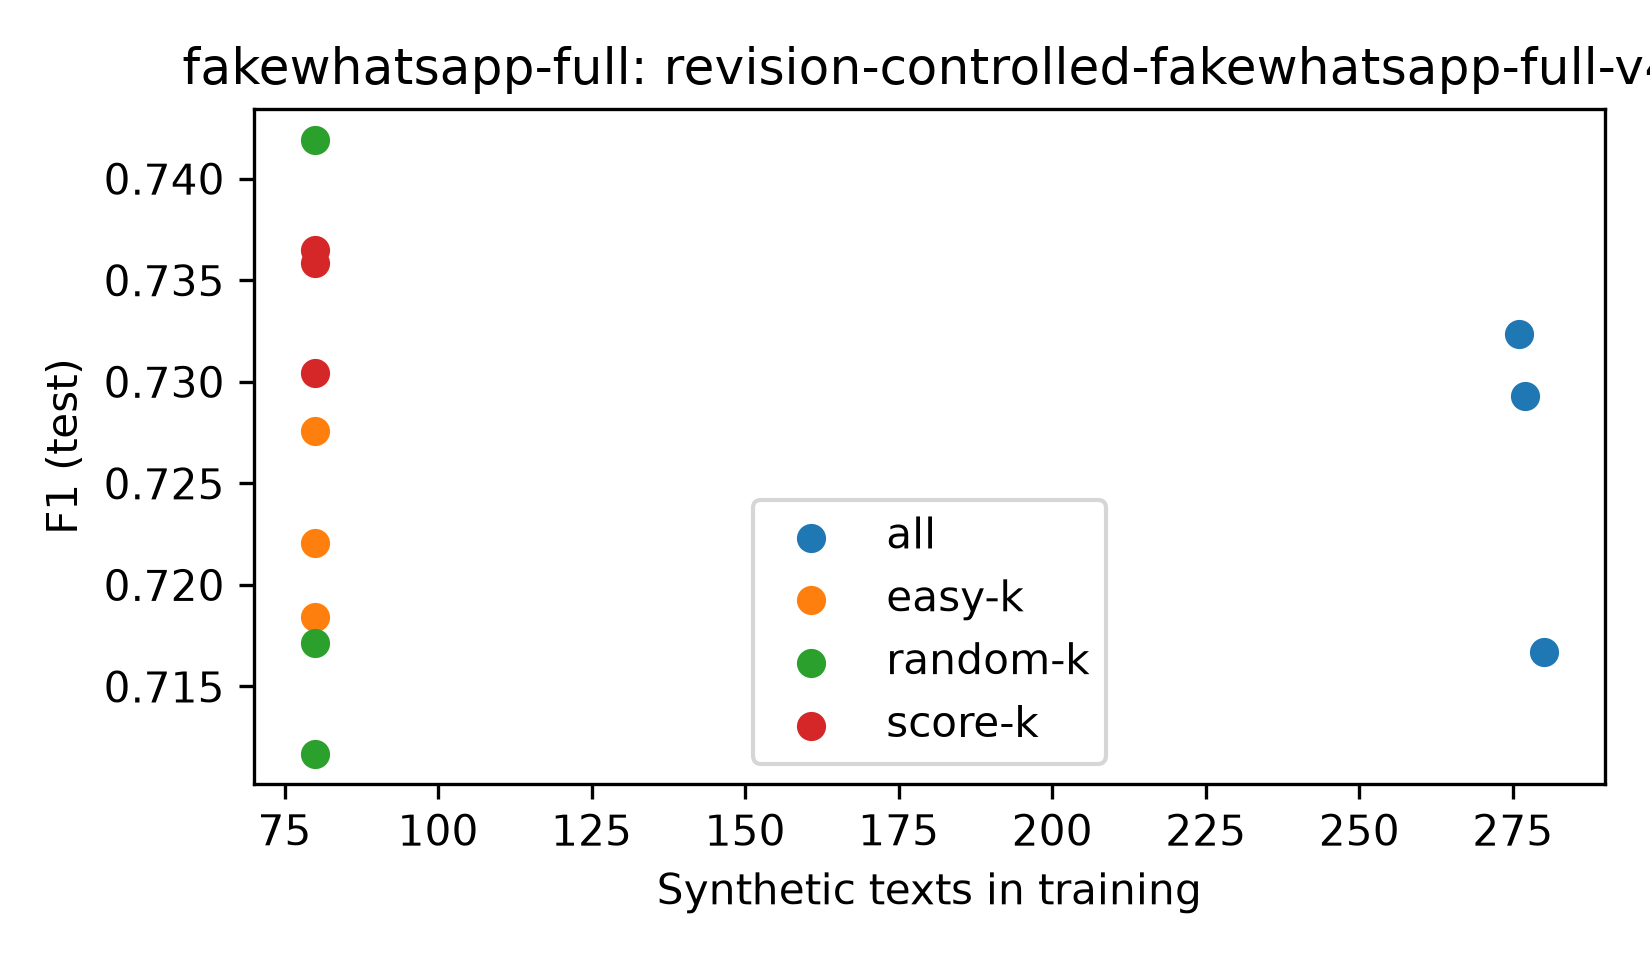
\includegraphics[width=.98\textwidth]{revision-controlled-fakewhatsapp-full-v4-fakewhatsapp-full-f1-vs-n_synthetic-20261023T003526Z.png}
\caption{F1 $\times$ número de sintéticos no treino (full). A curadoria de 80 textos atinge ou supera o uso de todos os 277 candidatos.}
\label{fig:pareto}
\end{figure*}

\begin{figure*}[t]
\centering
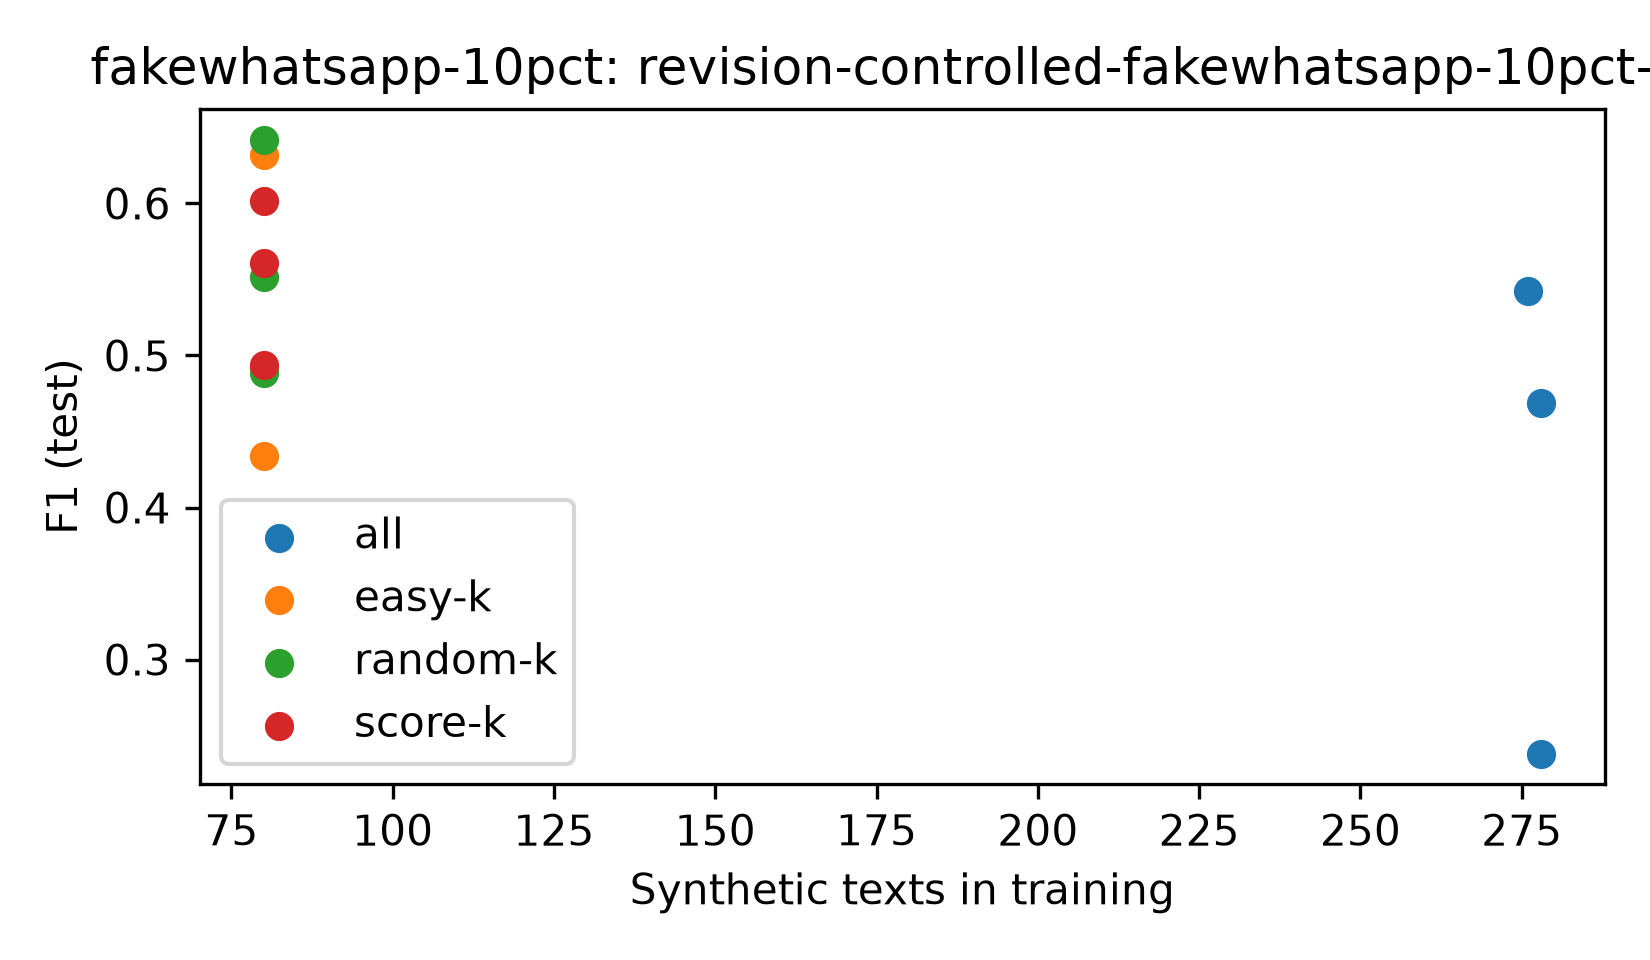
\includegraphics[width=.48\textwidth]{revision-controlled-fakewhatsapp-10pct-v4-fakewhatsapp-10pct-f1-vs-n_synthetic-20261023T003530Z.png}
\hfill
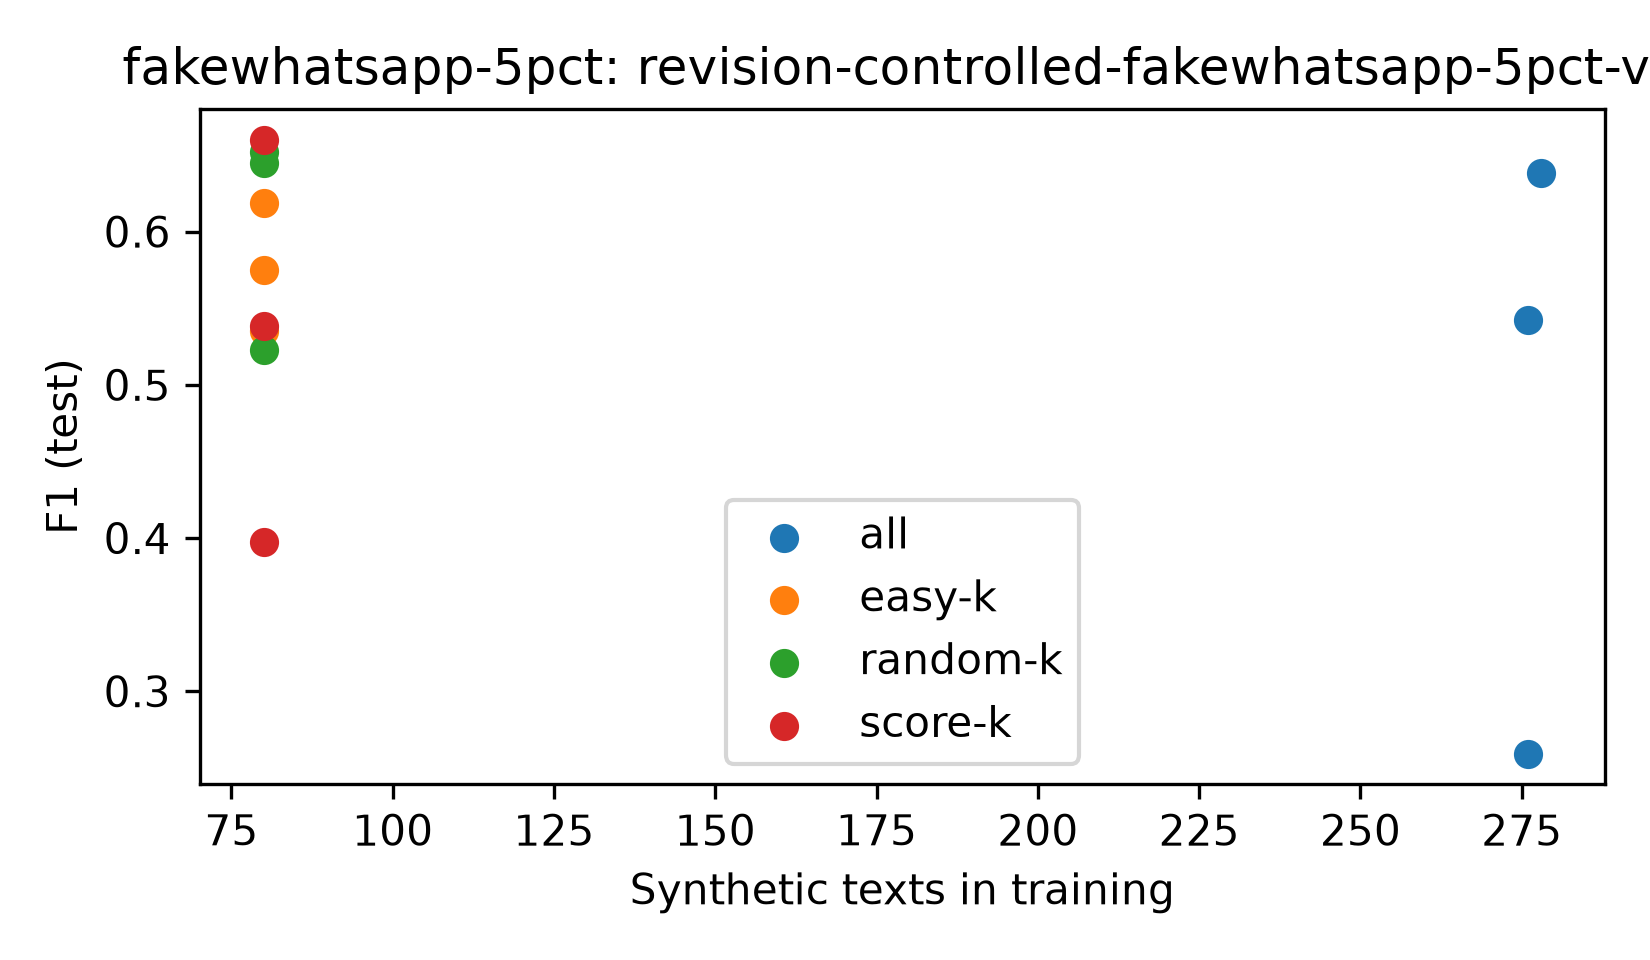
\includegraphics[width=.48\textwidth]{revision-controlled-fakewhatsapp-5pct-v4-fakewhatsapp-5pct-f1-vs-n_synthetic-20261023T003531Z.png}
\caption{F1 $\times$ número de sintéticos sob escassez (10\% à esquerda, 5\% à direita). Random-16 supera Score-16 e All em ambos.}
\label{fig:pareto-scarce}
\end{figure*}

Um classificador logístico (TF-IDF unigramas+bigramas, split aleatório) separa texto real de sintético com AUC $\approx 1{,}0$ em todos os cenários e braços. Isso quantifica o atalho estilístico, mas \emph{não} mede veracidade nem generalização temporal; o prompt v4 ainda vaza marcadores como ``fictícia'' e ``inventada'', que podem inflar a separabilidade.

\section{Discussão}

A versão anterior atribuía ganho ao score, mas não havia o controle aleatório. Com os mesmos candidatos, o score não supera o sorteio: o efeito relevante é \textbf{herdar pouco} (80 em vez de 277) e \textbf{calibrar o treino} (ponderação e limiar). O gate por erro/incerteza/diversidade permanece útil como filtro de redundância, mas não é a fonte do ganho de desempenho.

O \emph{Easy-}k (inversão do Profile2Gen) não supera consistentemente, então a hipótese de ``herdar os difíceis'' não foi confirmada neste domínio. A seleção por faixa de dificuldade intermediária fica como ablação futura, condicionada a checagem humana de rótulo.

\section{Limitações e Próximos Passos}

Três seeds (exploratório); rótulos sintéticos presumidos sem checagem factual humana; Fake.br ausente (pré-processamento exato indisponível); marcadores vazados no prompt v4. Próximos passos: (i) 10 seeds confirmatórias antes de olhar o holdout final; (ii) validação humana dos sintéticos; (iii) corpus raw ou pipeline exato do Fake.br; (iv) ablação de faixa de dificuldade; (v) trabalhos relacionados posicionando o estudo em ZeroGen/ProGen, active learning e dataset cartography~\cite{swayamdipta2020,settles2012}.

\section{Conclusão}

O ActiveInheritance, sob protocolo controlado, funciona como \textbf{curadoria de volume e calibração}, não como superioridade do score. Dados os mesmos candidatos, selecionar por erro/incerteza/diversidade não supera a seleção aleatória; e o colapso de recall sob escassez era majoritariamente limiar fixo e desbalanceamento. Esta revisão delimita onde a herança ativa ajuda---e onde o ganho não é atribuível à função de seleção.

\balance
\footnotesize
\begin{thebibliography}{00}

\bibitem{souza2025}
M.~D. de Souza and C.~Zanchettin, ``Breaking the Barrier of Hard Samples: A Data-Centric Approach to Synthetic Data for Medical Tasks,'' in \emph{Proc. ICML}, 2025.

\bibitem{monteiro2018}
R.~Monteiro, R.~Santos, T.~Pardo, T.~de Almeida, E.~Ruiz, and O.~Vale, ``Contributions to the Study of Fake News in Portuguese: New Corpus and Automatic Detection Results,'' in \emph{Proc. PROPOR}, 2018.

\bibitem{cabral2021}
L.~Cabral et al., ``FakeWhatsApp.Br: NLP and Machine Learning Techniques for Misinformation Detection in Brazilian Portuguese WhatsApp Messages,'' in \emph{Proc. ICEIS}, 2021.

\bibitem{souza2020}
F.~Souza, R.~Nogueira, and R.~Lotufo, ``BERTimbau: Pretrained BERT Models for Brazilian Portuguese,'' in \emph{Proc. BRACIS}, 2020.

\bibitem{shumailov2024}
I.~Shumailov et al., ``AI Models Collapse When Trained on Recursively Generated Data,'' \emph{Nature}, vol.~631, 2024.

\bibitem{swayamdipta2020}
S.~Swayamdipta, R.~Schwartz, N.~Lourie, Y.~Wang, H.~Hajishirzi, N.~A.~Smith, and Y.~Choi, ``Dataset Cartography: Mapping and Diagnosing Datasets with Training Dynamics,'' in \emph{Proc. EMNLP}, 2020.

\bibitem{settles2012}
B.~Settles, \emph{Active Learning}, ser. Synthesis Lectures on Artificial Intelligence and Machine Learning. Morgan \& Claypool, 2012.

% TODO(verificar): acrescentar ZeroGen e ProGen (Ye et al., EMNLP 2022) e SunGen;
% confirmar autores/veículo antes de submeter. Não citar sem verificar.

\end{thebibliography}

\end{document}
